%- block legend

Kurt estava em uma missão espacial em sua nave quando foi atacado por uma tropa de $N$ alienígenas invasores! Os alienígenas fizeram um cerco ao redor da nave de Kurt para impedir que ele consiga escapar para seu planeta natal. O plano deles é fazer com que Kurt fique preso em sua nave até que eventualmente fique sem oxigênio.

\begin{center}
    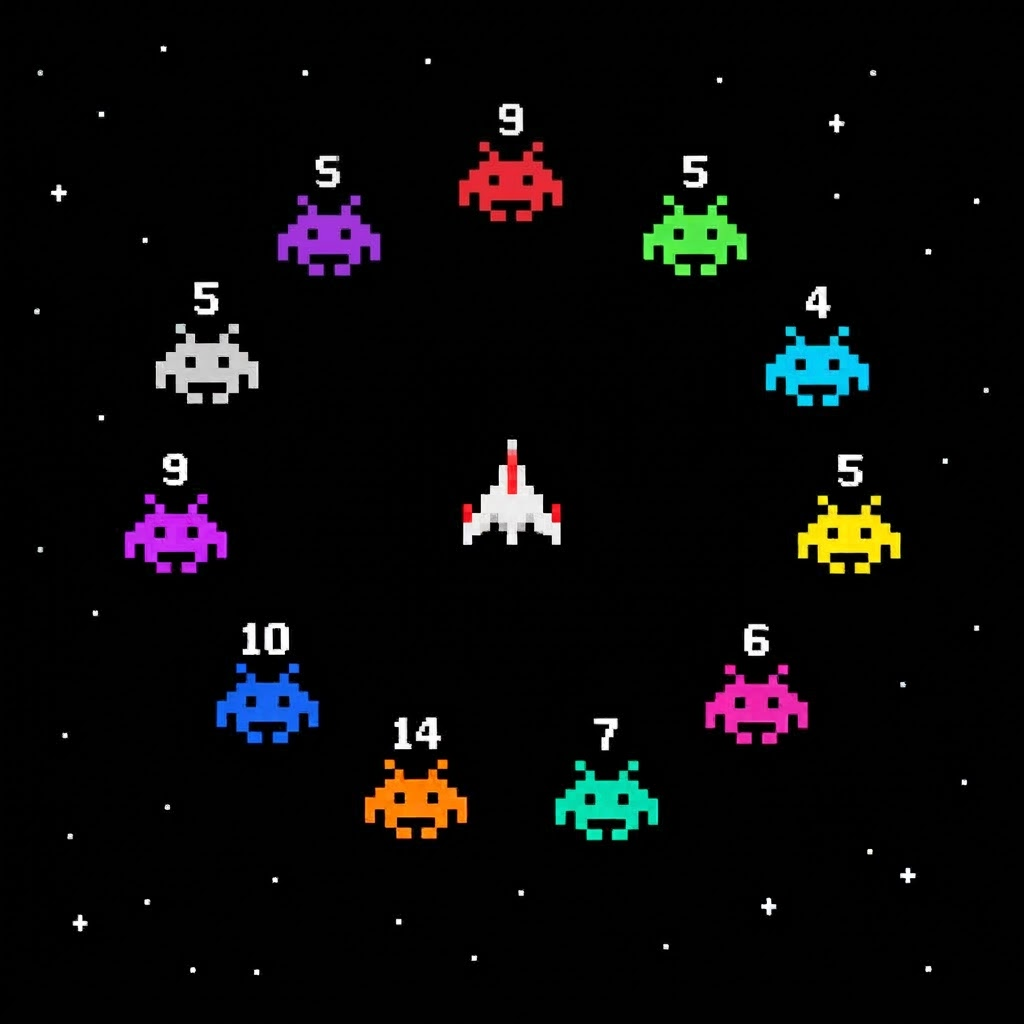
\includegraphics[scale=0.18]{space.png}
\end{center}

O que os alienígenas não contavam é que a nave de Kurt possui um poderoso mecanismo de defesa chamado \textit{Raio Pulverizador}.
Kurt conhece as defesas dos alienígenas. Cada alienígena possui um escudo de defesa de um determinado tipo. O $i$-ésimo alienígena possui um escudo do tipo $A_i$, onde $A_i$ é um número inteiro.

Apesar de poderoso, o Raio Pulverizador possui algumas limitações. O raio consegue pulverizar um conjunto de alienígenas de, no máximo, $K$ tipos distintos de escudo. Caso o disparo atinja um conjunto de alienígenas que possuam mais de $K$ tipos distintos de escudo, o raio irá ricochetear e retornar para a nave de Kurt, destruindo-a.
Além disso, o raio só pode ser disparado uma única vez. Depois de atingir o primeiro alienígena, o raio deve continuar seu trajeto atingindo apenas alienígenas adjacentes ao último alienígena atingido. Dessa forma, o disparo deve atingir uma sequência contínua de alienígenas, sem poder pular nenhum alienígena entre dois alvos consecutivos. O disparo pode seguir em qualquer uma das duas direções ao redor do círculo.

Dado o posicionamento dos alienígenas e os tipos de seus escudos, determine a maior quantidade de alienígenas que Kurt pode pulverizar com um único disparo sem destruir sua própria nave.
Formalmente, ajude Kurt a encontrar o tamanho da maior sequência contínua de alienígenas adjacentes que possui no máximo $K$ tipos distintos de escudo.
%- endblock

%- block input
A primeira linha contém dois inteiros $N$ e $K$ ($1 \leq N,K \leq 10^5$). A segunda linha contém $N$ inteiros $A_1,A_2,\ldots,A_N$ ($1 \leq A_i \leq 10^5$). O valor $A_i$ representa o tipo de escudo do $i$-ésimo alienígena. Os alienígenas estão dispostos em círculo, de modo que os alienígenas $1$ e $N$ são adjacentes.
%- endblock

%- block output
Imprima um único inteiro representando a maior quantidade de alienígenas que Kurt pode pulverizar em um único disparo do Raio Pulverizador.
%- endblock

%- block explanation_0
Neste exemplo, ilustrado anteriormente no enunciado, observamos que a sequência de alienígenas com tipos de escudos $[9,5,5,9,5,4,5]$ possui apenas 3 tipos distintos de escudos (4, 5 e 9), sendo essa a maior sequência de alienígenas que Kurt pode pulverizar.
%- endblock

%- block explanation_1
Neste exemplo, existem entre os 8 alienígenas apenas 6 tipos de escudos (1, 4, 8, 9, 12 e 15), logo Kurt pode pulverizar todos os alienígenas.
%- endblock

%- block editorial
Para resolver o problema, podemos inicialmente transformar o círculo de alienígenas em uma sequência linear duplicando seus elementos, permitindo considerar também as sequências que atravessam a fronteira entre o último e o primeiro alienígena. Em seguida, utilizamos a técnica de \textit{Two Pointers}
para manter uma sequência contínua e verificar quantos tipos distintos de escudo estão presentes nela. Sempre que a quantidade de tipos distintos ultrapassar $K$, diminuímos o tamanho da sequência pelo início até que ela volte a ser válida. Dessa forma, conseguimos encontrar a maior sequência contínua que possui no máximo $K$ tipos distintos de escudo. Como uma sequência válida não pode possuir mais de $N$ alienígenas, limitamos a resposta final a $N$.

Referência \textit{Two Pointers}: \url{https://usaco.guide/silver/two-pointers?lang=cpp}

Complexidade: $O(N)$
%- endblock
